\subsection{Módulo Existente e Hipóteses de Limitações}
\label{subsec:existent_module_and_limitations}

Assim como descrito anteriormente, o módulo de contagem de pessoas do dispositivo IoT configura os sensores utilizados para coleta dos dados, bem como a lógica empregada na aquisição e processamento das informações. Seu  principal objetivo, é comunicar ao sistema a entrada ou saída de qualquer indivíduo em uma instalação que possua um dispositivo IoT. Comumente, sistemas de software IoT baseiam-se na coleta periódica de informações, como forma de realizar o monitoramento, isto resulta na obtenção de um conjunto de dados que devem permitir a caracterização dos fenômenos em observação, neste caso, a entrada ou saída de pessoas em uma instalação.

O módulo de sensoriamento para contagem de pessoas, é composto por dois sensores ultrassônicos HC-SR04, que possuem invólucro e estrutura construída através de manufatura aditiva (impressão 3D). Estes sensores ficam posicionados acima da porta da instalação onde deseja-se contabilizar o fluxo de pessoas, assim como apresentado na Figura \ref{fig:count_people_module}. Os sensores ultrassônicos são capazes de coletar medidas acerca da distância entre eles e indivíduos ou objetos que estejam abaixo deles, e dentro do raio de alcance do seu emissor e receptor de ondas, possibilitando o monitoramento do ambiente desejado.

\begin{figure}[H]
    \center
    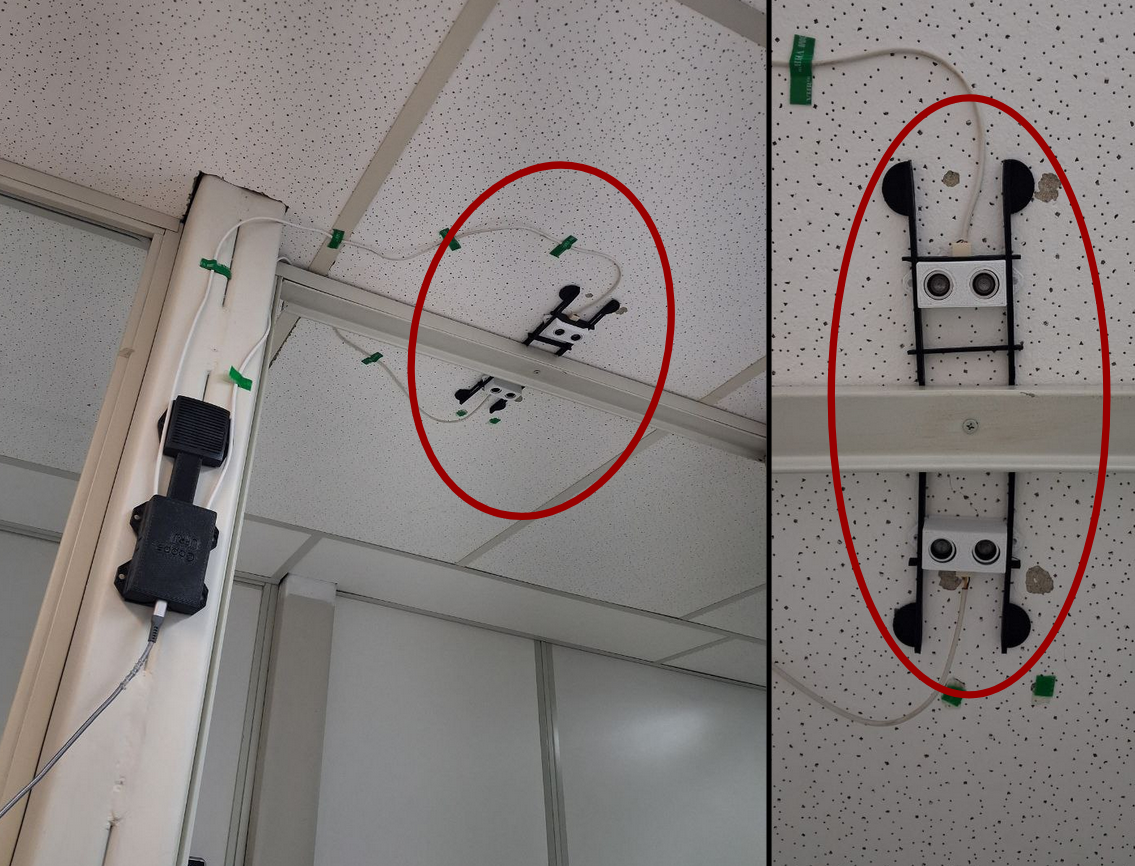
\includegraphics[scale=0.3]{images/count_people_module.png}
    \caption{Módulo de Sensoriamento para Contagem de Pessoas}
    \label{fig:count_people_module}
\end{figure}

O primeiro algoritmo proposto, para monitorar a quantidade de indivíduos em uma instalação baseia-se principalmente na disposição dos sensores ultrassônicos, que pode ser observada na Figura \ref{fig:count_people_module}, e no caráter periódico da coleta de dados pelo dispositivo IoT. Por este motivo, para cada evento de entrada ou saída, a sequência de dados coletados possui padrões bem definidos de ativação dos sensores. No caso de uma entrada, o sensor externo será ativado antes do sensor interno, bem como será o primeiro a ser desativado, para eventos de saída, o contrário acontece. Deste modo, o rastreamento de eventos de interesse, torna-se uma tarefa de identificação de padrões de ativação dos sensores.

Para lidar com este objetivo, o algoritmo construído consiste primeiramente na binarização dos dados coletados através de um limite preestabelecido, para que os estados dos sensores (ativado ou desativado) sejam diferenciados, assim como apresentado no Algoritmo \ref{alg:people_counting}. Após a binarização, o algoritmo compara o estado atual(tupla constituída pelo valor binarizado de cada sensor) com o estado anterior, para identificar e armazenar toda mudança de estado. Este novo estado, é armazenado em uma janela deslizante de tamanho fixo e a última tupla armazenada é descartada. Por fim, para cada novo estado, o algoritmo realiza a comparação entre a janela deslizante e os padrões de entrada e saída, buscando caracterizar e contabilizar eventos de interesse. Todos este fluxo pode ser visualizado através do Algoritmo \ref{alg:people_counting}.


% ------------------------------------------------------------
% No corpo do documento:


\begin{algorithm}[H]
\caption{Lógica Inicial Para Contagem de Pessoas}
\label{alg:people_counting}
\begin{algorithmic}[1]

\Function{COMPARAR\_VETORES}{$A,\;B$}
  \State \Comment{$A$ e $B$ são vetores}
  \If{$|A| \ne |B|$}  \Comment{Compara se os vetores possuem o mesmo tamanho}
    \State \Return \textbf{false}
  \EndIf

	\For{$i \gets 1$ \textbf{to} $|A|$} \Comment{Compara o valor de cada item dos vetores}
    \If{$A[i] \ne B[i]$}
      \State \Return \textbf{false}
    \EndIf
  \EndFor

	\State \Return \textbf{true} \Comment{Verdadeiro caso os vetores sejam iguais}
\EndFunction

\vspace{0.8em}

\Function{CALCULAR\_NUMERO\_DE\_PESSOAS}{$M$}
  \State $PADRAO\_DE\_ENTRADA$ \gets $[(0,0),(0,1),(1,1),(1,0),(0,0)]$
  \State $PADRAO\_DE\_SAIDA$ \gets $[(0,0),(1,0),(1,1),(0,1),(0,0)]$
  \State \Comment{$M$ é o vetor de medidas brutas}
	\State $estado\_do\_sensor \gets (s_{interno},s_{externo})$ \Comment{Vetor que armazena o estado atual binarizado}
  \State $entrada \gets 0$
  \State $saida \gets 0$
  \State $TOLERANCIA \gets 60$ \Comment{Limite para a binarização}
  \State $W \gets [(0,0),(0,0),(0,0),(0,0),(0,0)]$ \Comment{Vetor para o espaço de estados}

  \For{\textbf{each} $m \in M$}
    \State \Comment{--- Etapa de binarização das medidas brutas---}
    \If{$m.distancia\_sensor\_interno < TOLERANCIA$}
      \State $s_{interno} \gets 1$
    \Else
      \State $s_{interno} \gets 0$
    \EndIf

    \If{$m.distancia\_sensor\_externo < TOLERANCIA$}
      \State$s_{externo} \gets 1$
    \Else
      \State $s_{externo} \gets 0$
    \EndIf

    \State \Comment{--- Etapa de construção do padrão de bits capturado ---}
    \If{\textbf{not} \Call{COMPARAR\_VETORES}{$estado\_do\_sensor,\;W[5]$}}
      \State \Call{SHIFT\_LEFT}{$W$} \Comment{Descarta estado antigo}
      \State $W[5] \gets estado\_do\_sensor$ \Comment{Armazena o novo estado na última posição}

      \State \Comment{--- Etapa de identificação do evento de interesse ---}
      \If{\Call{COMPARAR\_VETORES}{$W,\;PADRAO\_DE\_ENTRADA$}}
        \State $entrada \gets entrada + 1$
      \ElsIf{\Call{COMPARAR\_VETORES}{$W,\;PADRAO\_DE\_SAIDA$}}
        \State $saida \gets saida + 1$
      \EndIf
	\State \Comment{Padrões inválidos não geram contagem}
    \EndIf
  \EndFor

  \State \Return $(entrada, saida)$
\EndFunction

\end{algorithmic}
\end{algorithm}

A lógica existente no Algoritmo \ref{alg:people_counting} faz uso da discretização dos dados e análise de mudança de estados dos sensores, para realizar tarefa de contagem de indivíduos por meio da coleta de medidas com sensores ultrassônicos, essas são ideias centrais para este tipo de atividade. No entanto, a abordagem descrita apresentou problemas durante testes práticos de funcionalidade, tendo como principal fator de seu mal funcionamento, a inexistência de uma etapa de pré-tratamento das medidas coletadas. 

Sendo assim, qualquer ruído de leitura pode induzir o sistema a gerar um estado incorreto, invisibilizando eventos de interesse e resultando em um monitoramento impreciso acerca da contagem de indivíduos em uma instalação. Ademais, o sistema de software IoT SAFE/UFRJ, tem como uma de suas principais características, a utilização de sensores de baixo custo, para construção dos dispositivos encarregados de realizar a coleta de dados \cite{SAFE-IOT}, esta categoria de sensor tende a ser mais imprecisa e ruidosa \cite{Komorowski2016}, por este motivo o sistema deve ser resiliente a este tipo de problema.

Antes de tratar ruídos e valores discrepantes (\textit{outliers}), é necessário compreender o verdadeiro gerador deste tipo de informação. Isto se faz necessário, pois este tipo de dado pode fornecer informações úteis para a etapa de modelagem do problema, bem como a exclusão de informações importantes de forma errônea pode comprometer todo o conjunto de dados inserindo viés ou simplesmente desperdiçando informações importantes \cite{Komorowski2016}. Logo, a segunda etapa do processo de evolução do módulo de contagem de pessoas, consiste na coleta e análise exploratória dos dados, para que se possa compreender e reconhecer os padrões naturais presentes na informação coletada \cite{Komorowski2016}.


